 Model analýzy, \textbf{zkoumá specifikované požadavky} z pohledu objektů, které lze nalézt v problémové doméně. \textbf{Kvalita} výsledného produktu je dána \textbf{mírou uspokojení požadavků zadavatele}. Právě otázka \textbf{korektní specifikace všech požadavků} bývá \textbf{problémem} všech softwarových systémů. Velmi často výsledek i mnohaletého úsilí týmu softwarových inženýrů propadne díky nedostatečné specifikaci zadání.

\subsection{Jazyk UML}
Slouží k \textbf{vytváření} výše uvedených \textbf{modelů vznikajících v průběhu realizace} požadovaného produktu.  V průběhu let se UML stal standardizovaným jazykem určeným pro vytvoření výkresové dokumentace (softwarového) systému. UML je jazyk umožňující \textbf{specifikaci}, \textbf{vizualizaci}, \textbf{konstrukci} a \textbf{dokumentaci} artefaktů softwarového systému. K vytváření jednotlivých modelů systému jazyk UML poskytuje celou \textbf{řadu diagramů} umožňujících \textbf{postihnout různé aspekty} systému. Jedná se celkem o \textbf{čtyři} \textbf{základní} \textbf{náhledy} a k nim přiřazené diagramy:

\begin{enumerate}
	\item \textbf{Funkční náhled}
	\begin{enumerate}
		\item \textbf{Diagram případů užití} - popisující vztahy mezi aktéry a jednotlivými případy použití. 
	\end{enumerate}
	\item \textbf{Logický náhled}
	\begin{enumerate}
		\item \textbf{Diagram tříd} - specifikující množinu tříd, rozhraní a jejich vzájemné vztahy. Tyto diagramy slouží k vyjádření statického pohledu na systém.
		\item \textbf{Objektový diagram}
	\end{enumerate}
	\item \textbf{Dynamický náhled popisující chování}
	\begin{enumerate}
		\item \textbf{Stavový diagram} - dokumentující životní cyklus objektu dané třídy z hlediska jeho stavů, přechodů mezi těmito stavy a událostmi, které tyto přechody uskutečňují. 
		\item \textbf{Diagram aktivit} -  popisující podnikový proces pomocí jeho stavů reprezentovaných vykonáváním aktivit a pomocí přechodů mezi těmito stavy způsobených ukončením těchto aktivit. Účelem diagramu aktivit je blíže popsat tok činností daný vnitřním
		mechanismem jejich provádění. 
		\item \textbf{Interakční diagramy}
		\begin{enumerate}
			\item \textbf{Sekvenční diagramy} -  popisující interkace mezi objekty z hlediska jejich časového uspořádaní.
			\item \textbf{Diagramy spolupráce} -  je obdobně jako předchozí sekvenční diagram zaměřen na interkace, ale z pohledu strukturální organizace objektů. Jinými slovy není primárním aspektem časová posloupnost posílaných zpráv, ale \textbf{topologie rozmístění objektů}. 
		\end{enumerate}
	\end{enumerate}
	\item \textbf{Implementační náhled}
	\begin{enumerate}
		\item \textbf{Diagram komponent} - ilustrující organizaci a závislosti mezi softwarovými komponentami. 
		\item \textbf{Diagram nasazení} - upřesněný nejen ve smyslu konfigurace technických prostředků, ale především z hlediska rozmístění implementovaných softwarových komponent na těchto prostředcích.
	\end{enumerate}
\end{enumerate}

\subsection{Specifikace požadavků}
Jazyk UML pro potřeby sestavení modelů \textbf{specifikace požadavků} využívá dvou typů diagramů: 
\begin{itemize}
\item \textbf{Diagram případů užití} popisující \textbf{vztahy} mezi \textbf{aktéry} a jednotlivými \textbf{případy použití}. 
\item \textbf{Sekvenční diagram} zobrazující \textbf{vzájemnou interakci} participujících \textbf{objektů} organizovanou podle časového hlediska. 
\end{itemize}
Cílem specifikace požadavků je \textbf{popsat co má softwarový systém dělat prostřednictvím specifikace jeho funkcionality}.  Modely specifikace požadavků slouží k odsouhlasení zadání mezi vývojovým týmem a zadavatelem.


\subsection{Diagram případů užití}
Modely, které jsou v rámci specifikace činností vytvářeny vychází z tak zvaných \textbf{případů užití} (\textbf{Use Cases}) tvořených: 
\begin{itemize}
\item \textbf{Aktéry} definující \textbf{uživatele} či \textbf{jiné systémy}, kteří budou vstupovat do interakce s vyvíjeným softwarovým systémem.
\item \textbf{Případy užití} specifikující vzory chování realizovaných softwarovým systémem.  Každý případ užití lze chápat jako \textbf{posloupnost vzájemně navazujících transakcí} vykonaných \textbf{v dialogu mezi aktérem a vlastním softwarovým systémem}.
\end{itemize}
\textbf{Účelem} diagramu případů užití \textbf{je definovat co existuje vně vyvíjeného systému} (\textbf{aktéři}) a \textbf{co má být systémem prováděno (případy užití)}. Vstupem pro sestavení diagramu případů užití je \textbf{byznys model}, konkrétně modely podnikových procesů.  \textbf{Výsledkem} analýzy těchto procesů \textbf{je seznam požadovaných funkcí softwarového systému}, které podpoří nebo dokonce nahradí některé z uvedených aktivity cestou jejich softwarové implementace. \\
\noindent\makebox[\textwidth]{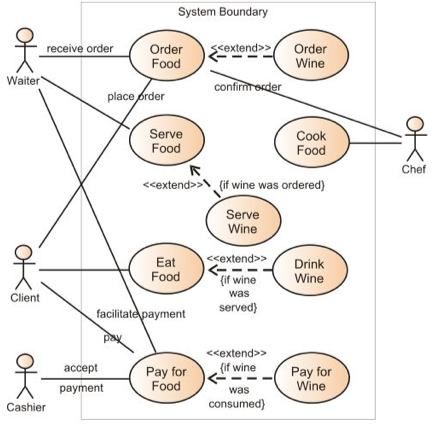
\includegraphics[width=13cm]{assets/usecase}}
Pro složitější a obsáhlejší diagramy případy užití se zavadí \textbf{tři typy vztahů mezi jednotlivými případy užití}:
\begin{itemize}
\item \textbf{Include} – případ užití může \textbf{obsahovat} jiný (UC s include se vždy provede před samotným UC).
\item \textbf{Extend} – případ užití může \textbf{rozšiřovat} jiný (UC s extend se může nebo nemusí provést).
\item \textbf{Generalization} – případ užití může být s\textbf{peciálním případem }jiného (dědičnost).
\end{itemize}


\subsection{Sekvenční diagram}
Jazyk UML poskytuje pro účely zaznamenání těchto \textbf{vzájmených intrakcí} tzv. sekvenční, někdy také nazývaný interakční, diagram. Tento diagram postihuje jaké \textbf{zprávy} (\textbf{požadavky}) \textbf{jsou mezi objekty zasílány} \textbf{z pohledu času}. Diagram je tvořen \textbf{objekty uspořádanými do sloupců} a šipky mezi nimi odpovídají {vzájemně si zasílaným zprávám}. Zprávy mohou být {synchronní} nebo {asynchronní}. V případě \textbf{synchronních zpráv odesílatel čeká na odpověď} (odezvu) adresáta, v případě \textbf{asynchronní zprávy odesílatel nečeká} na odpověď a pokračuje ve vykonávání své činnosti. Souvislé provádění nějaké činnosti se v sekvenčním diagram vyjadřuje svisle orientovaným obdélníkem. Odezvu adresáta lze opět modelovat, v tomto případě tzv. \textbf{návratovou zprávou (přerušovaná čára)}. Tok času probíhá ve směru od shora dolů.
\\\\
\noindent\makebox[\textwidth]{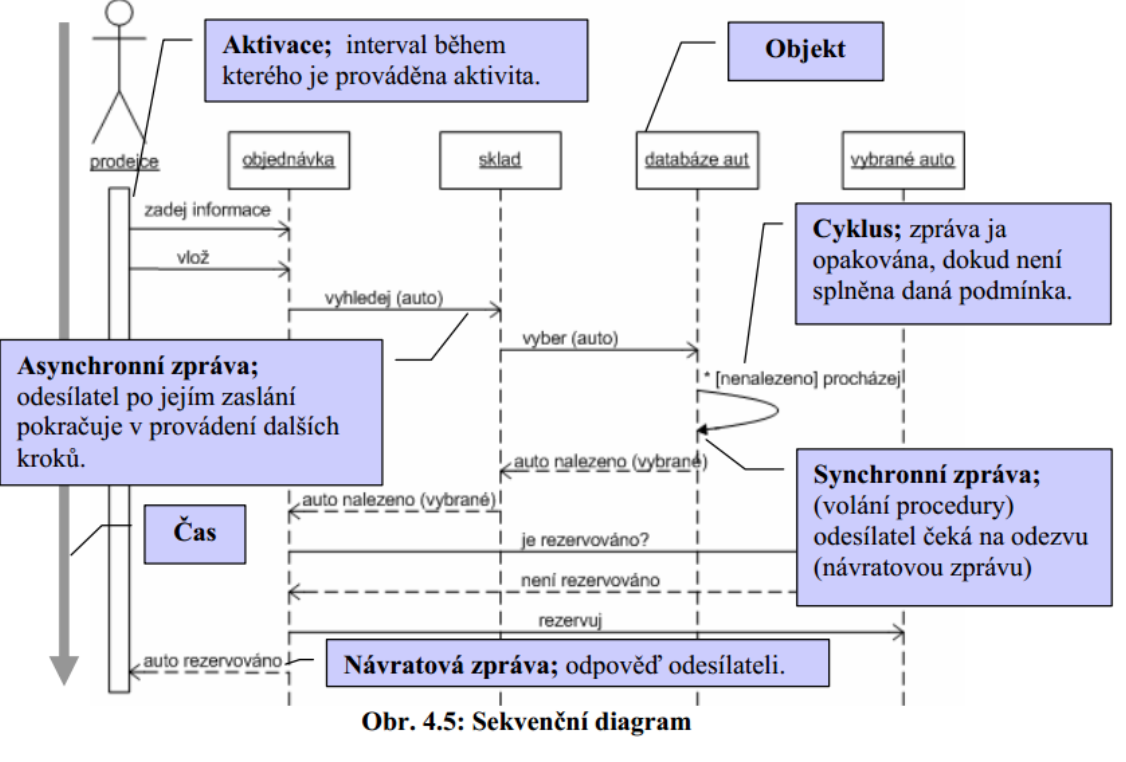
\includegraphics[width=\textwidth]{assets/sekv}}